\section{Introduction}
As robots increasingly enter our lives, mapping their impact becomes a primary challenge \cite{broadbent2017interactions, brondi2021we}. In addition to designing robots to serve a specific function \cite{goodrich2008human} and to be accepted by humans \cite{bishop2019social}, we also need to consider the social aspects that people automatically assign to interactions with them \cite{hoffman2014designing, erel2019robots, erel2021excluded, duffy2003anthropomorphism, novikova2014design}. Previous studies have examined how interacting with robots can lead to both positive \cite{tennent2019micbot, erel2022enhancing, adi2022non} and negative \cite{erel2021excluded, salomons2021minority, hitron2022ai} social effects, similar to those observed in human dynamics. Most of these studies focused on the impact of the robots' behavior and communication modalities (i.e., speech and gestures) while controlling for the robot's characteristics and design. However, one of the most significant advantages of robots as autonomous devices is the freedom in their design and the ability to adjust it to their specific function \cite{hoffman2014designing}. This suggests that robots are expected to employ varying design characteristics, including various forms, colors, sizes, and heights. These characteristics are already known to have a social impact in human-human interactions and human-social dynamics \cite{bartneck2018robots, bernotat2017shape, saerbeck2010perception, hiroi2008bigger}.


 \begin{figure}[t]
     \centering
     \vspace{0.2cm}
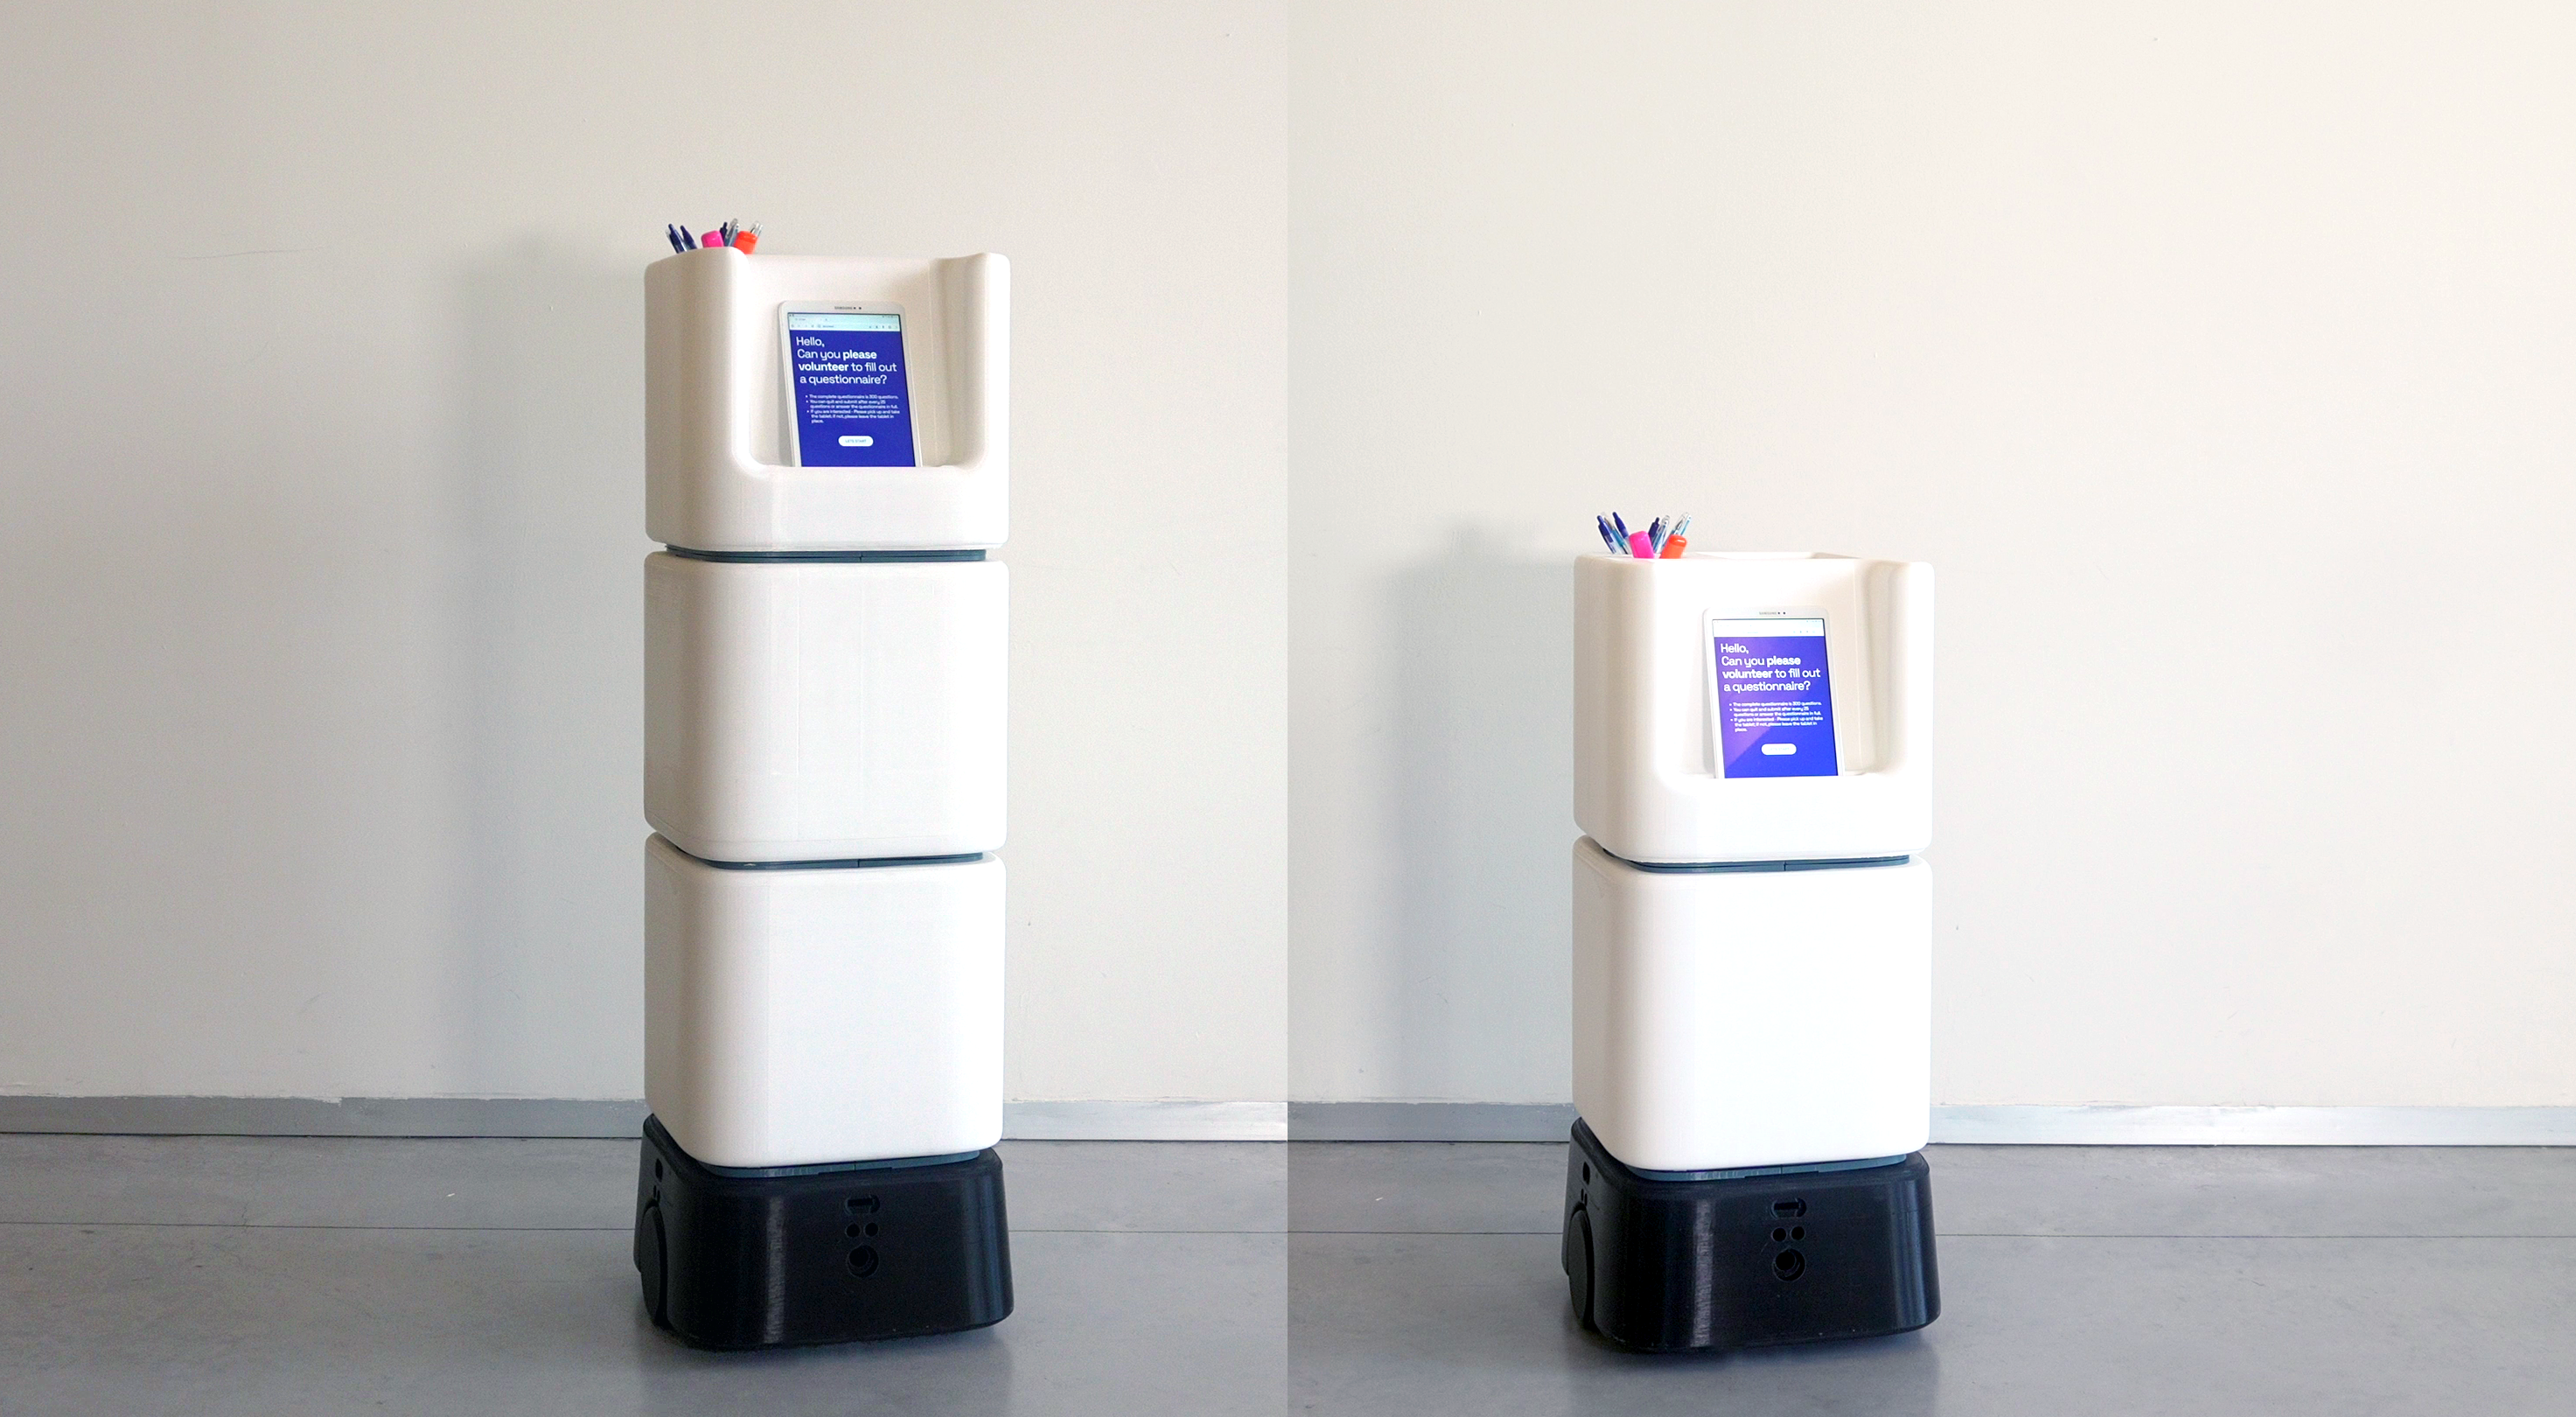
\includegraphics[width=1\linewidth]{Figures/MORPHY_RoMan_Tall-Short-Robot-SideBySide.png}
     \caption{The modular robotic service table: Short and Tall versions.}
     \label{fig:MORPHY - A Modular Robotic Platform}
  %   \vspace{-9pt}
 \end{figure}


Previous work suggests that robot design characteristics may also significantly impact social dynamics when interacting with them \cite{bartneck2018robots, bernotat2017shape, saerbeck2010perception}. People respond differently to robots based on their color \cite{bartneck2018robots}, gendered design cues (feminine vs. masculine) \cite{bernotat2017shape}, and motion style \cite{saerbeck2010perception}. Another interesting design characteristic is the robot's height. Previous studies indicated that it has a diverse impact on the social dynamics between the human and the robot \cite{hiroi2008bigger}, with some reporting similar effects to those observed with human height. A common finding in human-human interactions is that taller people are perceived as more competent, dominant, charismatic, persuasive, and likely to occupy positions of leadership and authority \cite{young1996height, jaeger2011thing,stogdill1948personal,stulp2013tall}. As a result, people tend to comply with taller people's requests \cite{young1996height, higham1992rise, stogdill1948personal}. Similarly, studies evaluating interactions with robots have shown that robots' height impacts compliance with the robot's operator, with taller robots leading to increased compliance \cite{rae2013influence} and trust \cite{gervasi2024does}. However, other studies indicated that people prefer to collaborate with short robots \cite{samarakoon2022review, walters2009preferences} and perceive the interaction with them as safer \cite{joosse2021appearance}. This points to a potential preference for shorter robots—opposite to the height-related effects seen in human-human interactions (where being taller is associated with leadership and charisma \cite{judge2004effect}).
A factor that may mediate the impact of robotic height is the human-likeness of the robot \cite{walters2009preferences}. As suggested earlier, one of the greatest advantages of robots is the ability to adjust their design to their intended function \cite{hoffman2014designing}. Accordingly, robots will take many forms, ranging from robots with a humanoid appearance to familiar objects and abstract objects. The automatic tendency to anthropomorphize even highly non-humanoid robots \cite{erel2019robots} suggests that height may influence social dynamics in HRI, regardless of the robot’s degree of human-likeness. Nevertheless, it is unclear if this social impact would parallel the effect of height in human-human interactions \cite{erel2024rosi}. While it is reasonable to assume that interactions with humanoid robots would follow similar patterns to those with other humans (see, for example, \cite{maj2024can}), it has yet to be explored if a similar pattern would emerge when interacting with highly non-humanoid robots. The robot's machine-like nature may mediate the social influence of the robot's height, leading to different and unique effects \cite{joosse2021appearance}. 
 
In this work, we designed and developed a robotic object (i.e., a mobile service table) to evaluate the impact of the robot's height on participants' willingness to comply with its request. The robotic object was designed as a modular platform composed of various modules that could be easily added or removed to change the robot's height. Using the flexibility offered by the platform, we could change the robot's height without changing other design features (see Figure \ref{fig:MORPHY - A Modular Robotic Platform}). We compared: (1) an interaction with a Short robot, composed of two modules and 95 cm height; (2) and an interaction with a Tall robot, composed of three modules and 132 cm height. In the experiment, participants performed a cognitive task on a computer. When done, they were informed that the experiment was complete. While waiting to receive their credits, the robotic platform entered the room, carrying a tablet with a call for voluntarily filling out a 300-question-long questionnaire \cite{soto2017next}. To test if the impact of the robot's height would parallel the effect of height in human-human interactions, we evaluated the compliance with the robot's request (i.e., the number of questions participants volunteered to answer) and the robot's perception. 


 \begin{figure*}[h]
     \centering
      \vspace{0.3cm}
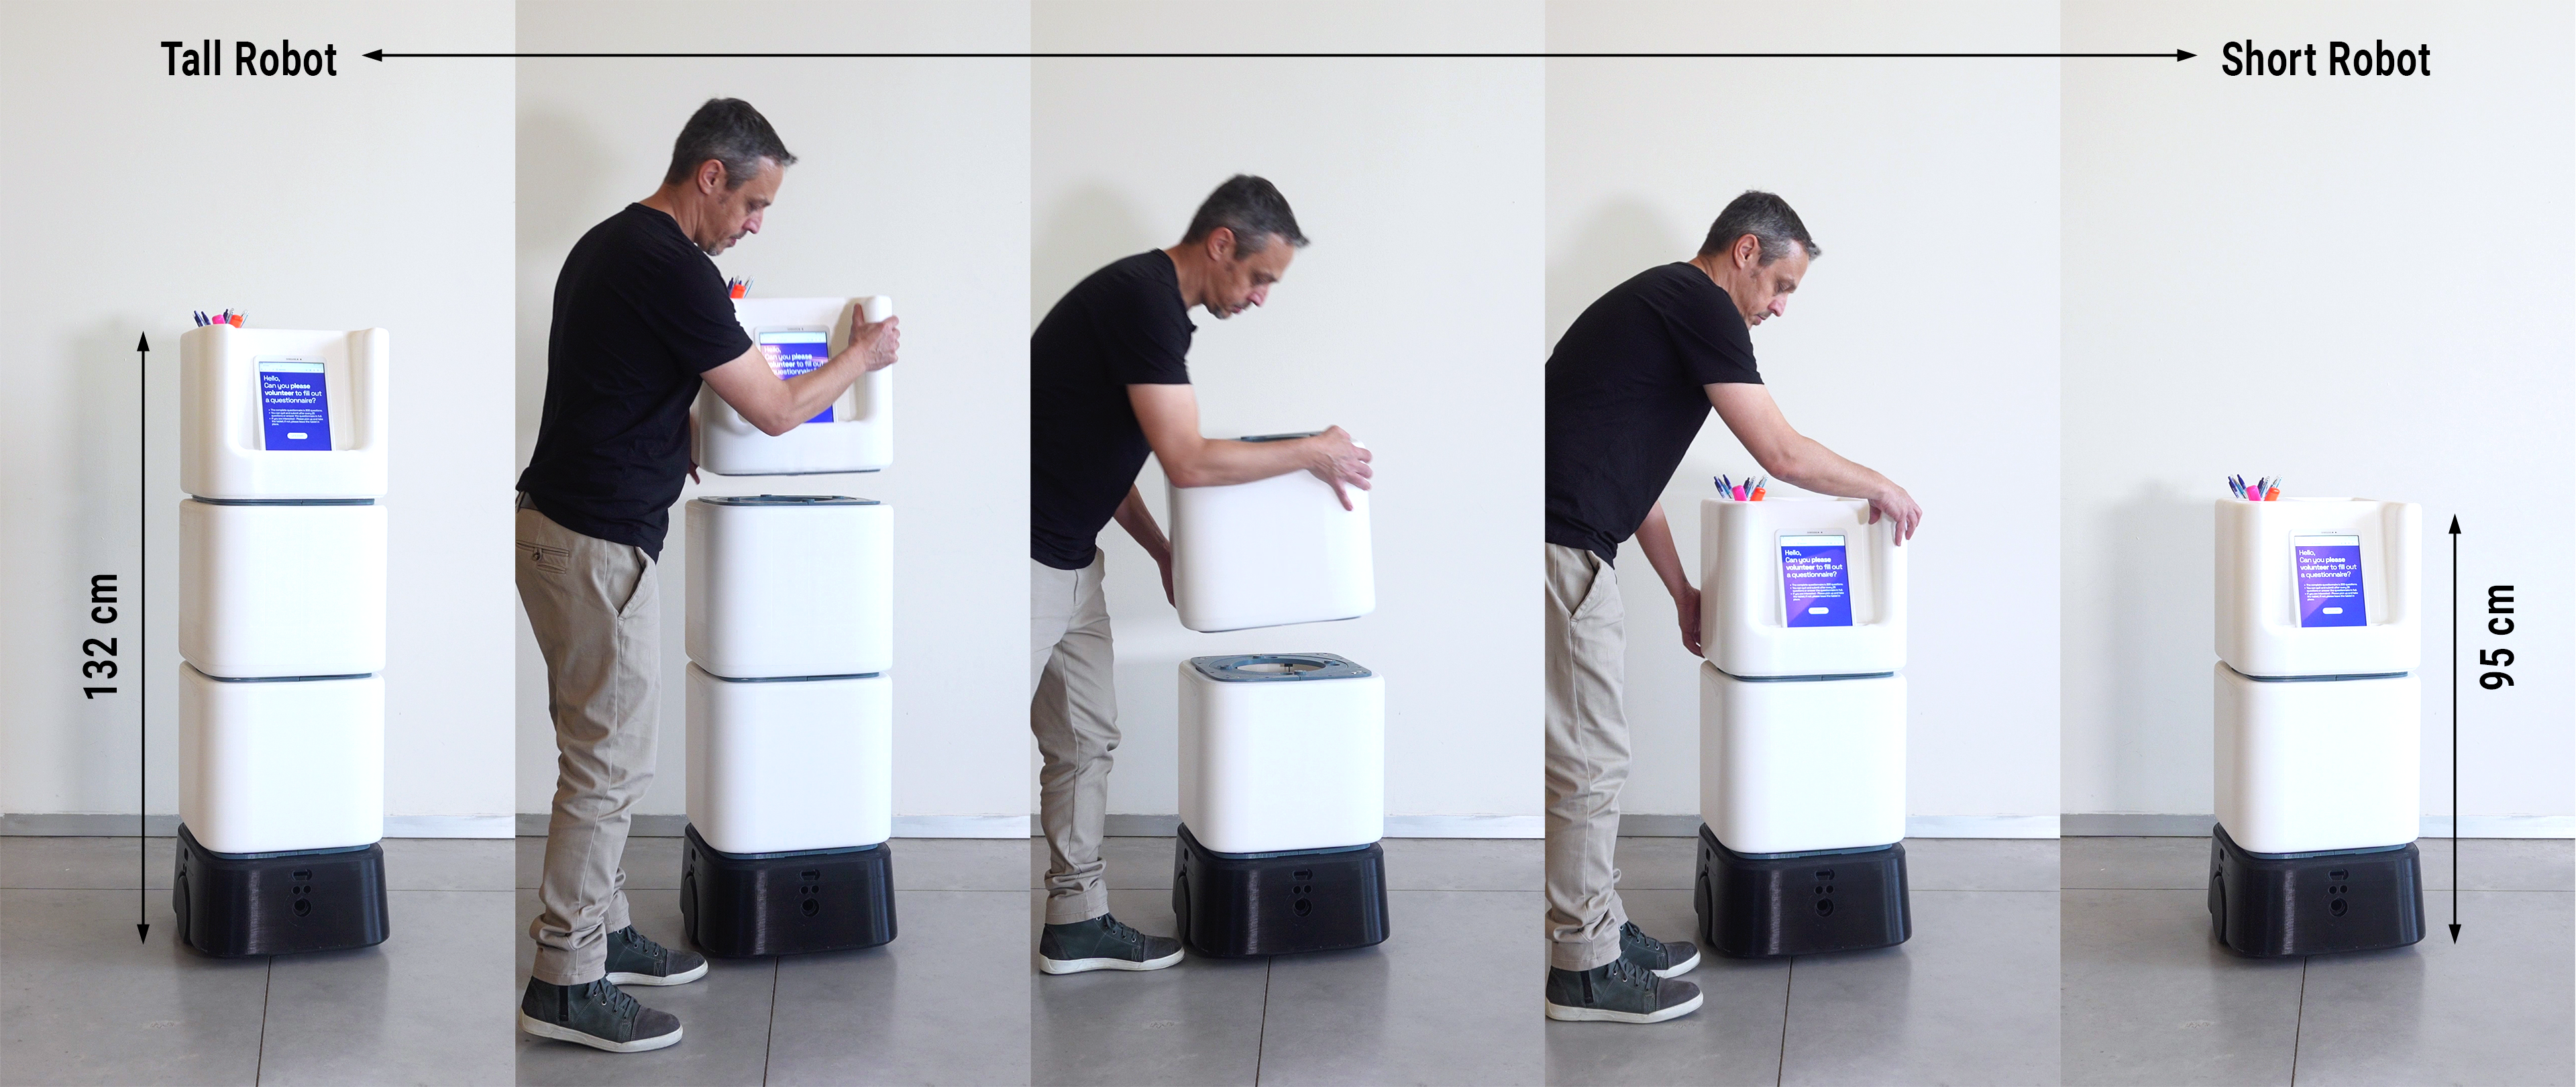
\includegraphics[width=0.85\linewidth]{Figures/MORPHY_RoMan_Assembly.png}
     \caption{From Tall to Short, and vice versa. Robot assembly.}
     \label{fig:robotfigure}
   % \vspace{-1em}
 \end{figure*}


%\begin{figure}
%  \includegraphics[width=\textwidth]{Figures/ISRA-HCI.png}
%  \caption{A. Low and high fidelity prototype; B. Root Assembly; C. Tall robot and Short robot; D. Top unit iterations}
 % \Description{A figure showing the robot design iteration}
 % \label{fig:robotfigure}
%\end{figure}








